%label:"fig:PushoffInFukayaSeidelCategory"
%type:"figure"
%name:"pushoff in Fukaya-Seidel category"
%caption:"To obtain transversality, the Lagrangian submanifolds in the Fukaya-Seidel category are pushed off one another with respect to the projection $W: Y \to \CC$."
%parent:"art_ASideLandauGinzburgModel"


    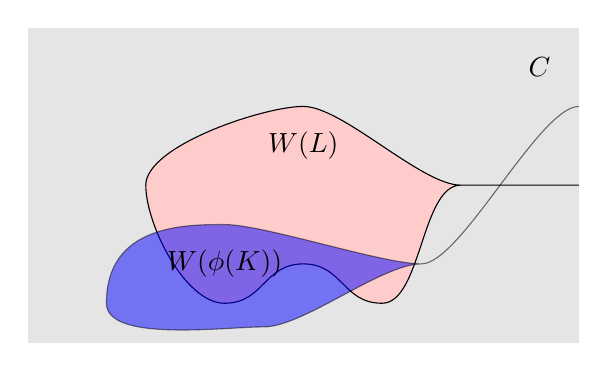
\begin{tikzpicture}

        \fill[gray!20] (-3,2.5) rectangle (4,-1.5);
        \draw[fill=red!20] (2.5,0.5) .. controls (2,0.5) and (1,1.5) .. (0.5,1.5) .. controls (0,1.5) and (-1.5,1) .. (-1.5,0.5) .. controls (-1.5,0) and (-1,-1) .. (-0.5,-1) .. controls (0,-1) and (0,-0.5) .. (0.5,-0.5) .. controls (1,-0.5) and (1,-1) .. (1.5,-1) .. controls (2,-1) and (2,0.5) .. (2.5,0.5) .. controls (4,0.5) and (3,0.5) .. (4,0.5);
        \node at (0.5,1) {$W(L)$ };
        \node at (3.5,2) {$\mathbb{C}$};
        \draw[fill=blue, opacity=.5] (-0.5,0) .. controls (-1,0) and (-2,0) .. (-2,-1) .. controls (-2,-1.5) and (-0.5,-1.3) .. (0,-1.3) .. controls (0.5,-1.3) and (1.5,-0.5) .. (2,-0.5) .. controls (2.5,-0.5) and (3.5,1.5) .. (4,1.5) .. controls (3.5,1.5) and (2.5,-0.5) .. (2,-0.5) .. controls (1.5,-0.5) and (0,0) .. (-0.5,0);
        \node at (-0.5,-0.5) {$W(\phi(K))$};
    \end{tikzpicture}

